\chapter{Crash course in complex analysis}\llabel{complex-analysis}
Complex analysis is calculus on the complex numbers. The main functions of study are complex differentiable functions.

Reference books: Lang or Ahlfors
\section{Holomorphic functions}
\begin{df}
Let $U\subeq \C$ be an open set and $f:U\to \C$ be a function. The \textbf{derivative} of $f$ is
\[
f'(z):=\lim_{\De z\to 0} \frac{f(z+\De z)-f(z)}{\De z}
\]
if it exists. $f$ is \textbf{holomorphic} if its derivative exists at every point of $U$. $f$ is \textbf{meromorphic} if it is defined and holomorphic on $U$ except at a discrete set of points.
\end{df}
Write $f(x+iy)=u(x,y)+iv(x,y)$. Note that $f$ being differentiable is a much {\it stronger} condition than being simply $u$ and $v$ being differentiable, because the limit of $f$ as $\De z\to 0$ along the real and complex directions must be equal:
\[
\pd ux+\pd vx = \rc{i} \pa{\pd uy +i\pd vy}.
\]
Thus we get the Cauchy-Riemann criteria: If $f$ is differentiable as a function of $(x,y)$, then $f$ is holomorphic iff
\[
\pd ux=\pd vy,\quad \pd uy =-\pd vx.
\]
Another way to think about complex differentiability is that holomorphic maps preserve angles (i.e. are {\it conformal}); we have
\[
f(z+re^{i\te}) -f(z)\approx re^{i\te} f'(z).
\]

Because complex differentiability is such a strong property, holomorphic functions have many nice properties. Hence it is often useful to take functions defined on the reals and extend them as far as possible on $\C$. Some of the good properties are the following (to be explained in the rest of the chapter); note they are not necessarily true for real differentiable functions!
\begin{itemize}
\item
A function is holomorphic iff it is analytic (has a power series expansion).
\item
A sequence of holomorphic functions with good convergence properties converges to a holomorphic function.
\item A bounded entire function is constant.
\item If two holomorphic functions agree on a set containing a limit point, then they are equal. Thus analytic continuations are unique.
\item Bounds on a function give bounds on the derivative. Hence we can ``differentiate" asymptotic formulas.
\item We can expand holomorphic functions into products or sums depending on their poles and zeros---in much the same way that rational functions can be expanded into partial fractions or factored.
\end{itemize}
\section{Complex integration}
We now give two definitions of the integral.
\begin{df}
A \textbf{path} is a continuous function $\ga:[a,b]\to \C$. It is called a \textbf{loop} if $\ga(a)=\ga(b)$.
Let $f$ be a holomorphic function on $U$ and $\ga$ be a path in $U$.
\begin{enumerate}
\item
If $\ga$ is differentiable (except possibly at a finite number of points), define
\[
\int_{\ga} f(z)\,dz = \int_a^b f(\ga(t)) \ga'(t)\,dt.
\]
\item
Define an (indefinite) \textbf{integral} of $f$ on a set $V$ to be a function $F$ on $V$ such that $F'(z)=f(z)$. Given holomorphic $f$, choose points $t_0,\ldots, t_n$ such that there exist open sets $U_j\supeq f(\ga([t_{j-1},t_j]))$ such that $f$ has an integral $F_j$ on $U_j$. Define
\[
\int_{\ga}f(z)\,dz=\sum_{k=1}^n [F_j(\ga(t_j))-F_j(\ga(t_{j-1})].
\]
\end{enumerate}
\end{df}
Note that unlike in the real case, indefinite integrals may not exist globally, for example, $\ln t$ is locally an integral for $\rc t$ but cannot be extended holomorphically to $\C\bs \{0\}$. We need to establish the well-definedness of the second definition.
\begin{thm}[Cauchy's Theorem, version 1]\llabel{cauchy1}
Let $f$ be holomorphic on a closed rectangle $R$, with boundary $\partial R$. Then (using the first definition),
\[
\int_{\partial R}f=0.
\]
\end{thm}
From this one can show that integrals exist locally by defining
\[
F(z)=\int_{z_0}^{z} f(s)\,ds
\]
where the integral is along horizontal and vertical lines; moreover one gets well-definedness in the second definition.

We can now define the logarithm of a function.
\begin{df}
Let $f$ be a holomorphic function on a simply connected set $U$ (see Definition~\ref{homotopic}), with $f(z)\ne 0$ on $U$. Choose $z_0\in U$ and $a_0$ such that $e^{a_0}=z_0$.
\[
(\ln f)(z)=\int_z^{z_0} \fc{f'}{f}(z)\,dz.
\]
\end{df}
Note different definitions of the logarithm will differ by integer multiples of $2\pi i$, and $e^{(\ln f)(z)}=f(z)$. The motivation comes from the fact that one would expect the derivative of $\ln f(z)$ to be $\fc{f'}{f}(z)$. We write $(\ln f)(z)$ to emphasize that this is {\it not} simply a composite of functions: We could have $f(z_1)=f(z_2)$ but $(\ln f)(z_1)\ne (\ln f)(z_2)$.\footnote{Consider, for example, the case where $f(z)=z^2$ on $\C\bs\R_{\le 0}$, and $z_1=i$, $z_2=-i$.}

We seek a generalization of Theorem~\ref{cauchy1} to meromorphic functions and arbitrary paths. 
\section{Cauchy's Theorem}
\begin{df}\llabel{homotopic}
Two paths $\ga$ and $\eta:[a,b]\to \C$ are \textbf{homotopic} if there exists a continuous map
\[
\ga_s(t):[0,1]\times [a,b]\to \C
\]
such that $\ga_0(t)=\ga(t)$ and $\ga_1(t)=\eta(t)$.

A subset of $\C$ is simply connected if it is pathwise connected and every loop in $\C$ is homotopic to a point.
\end{df}
\begin{thm}
Let $U$ be a simply connected open set containing $z_0$. 
Every path $\ga$ around $z_0$ in $U\bs\{z_0\}$ is homotopic to a circle going around $z_0$ $n$ times for some $n\in \Z$. This $n$ can be calculated by
\[
n=W(\ga,z_0):=\rc{2\pi i}\int_{\ga}\frac{f(z)}{z-z_0}\,dz
\]
and is called the \textbf{winding number}.
\end{thm}
\begin{thm}[Global Cauchy's formula]
Let $U$ be a simply connected open set and $f:U\to \C$ be holomorphic. Suppose $\ga$ is a loop in $U$. Then
\[
\rc{2\pi i}\int_{\ga} \fc{f(z)}{z-z_0}\,dz=W(\ga,z_0)f(z_0).
\]
\end{thm}
%$z_0\in D$, and $\ga$ be a circle around $f$ in $D$. Then
%\[
%f(z_0)=\rc{2\pi i} \int_{\ga} \frac{f(z)}{z-z_0}\,dz
%\]
%\end{thm}
%\begin{thm}
%Let $\ga$ be a closed chain in $U$. Define the \textbf{winding number} of $\ga$ with respect to $\al$ to be
%\[
%W(\ga,\al)=\rc{2\pi i}\int_{\ga} \rc{z-\al} \,dz.
%\]
%Suppose $\ga\sim 0$ in $U$ and $f$ is analytic on $U$. Then 
%\end{thm}
%Note: mention def'n of ln(f)! Mention differentiating asymptotic formulas.
\section{Power series and Laurent series}
As complex differentiability is a much stronger condition than differentiability for real functions, holomorphic functions enjoy nicer properties. The most important one is the following.
\begin{df}
A function $f:U\to \C$ is \textbf{analytic} at $z_0$ if it can be written as a power series in a neighborhood around $z_0$:
\[
f(z)=\sum_{n=0}^{\iy} a_n(z-z_0)^n.
\]
\end{df}
If $f$ is given by its power series representation then we must have $a_n=\frac{f^{(n)}(z)}{n!}$.
\begin{thm}
A function $f:U\to \C$ is analytic iff and only iff it is holomorphic.
\end{thm}
Note this is not true for real functions: for example, $e^{-\rc{x^2}}$ has Taylor expansion equal to 0 at 0, but is not the zero function. This kind of irregularity does not happen for holomorphic functions.
\begin{cor}
A holomorphic function has infinitely many derivatives.
\end{cor}
The following theorem says that for holomorphic functions, the radius of convergence is ``as large as it could possibly be."
\begin{thm}\llabel{radius-convergence}
Suppose $f$ is holomorphic on a disc $N_r(z_0)$ of radius $r$ around $z_0$. Then the Taylor series around $z_0$ converges absolutely to $f$ on $N_r(z_0)$.
\end{thm}
\begin{proof}
Estimate coefficients using Cauchy's theorem. Complex Analysis, Lang III.7.3.
\end{proof}
We can generalize power series to allow terms with negative exponents.
\begin{thm}
Suppose $f$ is defined on an annulus $A=\set{z}{r<|z-z_0|< R}$. Let $C$ be the circle of radius $r'\in(r,R)$ around $z_0$. Then $f$ has a Laurent expansion on $A$:
\[
f(z)=\sum_{n=-\iy}^{\iy} a_n(z-z_0)^n,\quad a_n=\rc{2\pi i}\int_{C} \frac{f(z)}{(z-z_0)^{n+1}}\,dz.
\]
If $f$ is defined on $\set{z}{|z-z_0|<R}$ then 
\[f^{(n)}(z_0)=\frac{n!}{2\pi i}\int_{C} \frac{f(z)}{(z-z_0)^{n+1}}\,dz.\]
\end{thm}
The coefficient $a_{-1}$ is called the \textbf{residue} of $f$ at $z_0$:
\[
\Res_{z_0}(f)=a_{-1}.
\]
The following theorem controls the size of the derivatives of a complex analytic function by its values of the function in a circle. Note that in the real analytic case we can't make such a statement!
\begin{cor}\llabel{cor:cauchy-ineq}
Suppose $f$ is defined on $\set{z}{|z-z_0|<R}$, and let $C$ be a circle of radius $r<R$ around $z_0$. Then 
\[
|f^{(n)}(z)|\le \frac{n!}{r^n} \max_{z\in C} f(z)
\]
and the $n$th coefficient in the power series expansion satisfies
\[
a_n\le \rc{r^n}\max_{z\in C} f(z).
\]
\end{cor}
\begin{proof}
Simply note that in the integral $\int_{C} \frac{f(z)}{(z-z_0)^{n+1}}\,dz$, the denominator has constant absolute value $r^{n+1}$, the numerator is bounded by $\max_{z\in C} f(z)$, and the arc length is $2\pi r$.
\end{proof}
\begin{cor}[Liouville]
A bounded entire function is constant.
\end{cor}
\begin{proof}
We can take $r\to \iy$ in the inequality for $n=1$ to find that $f'(z)=0$ everywhere.
\end{proof}

\subsection{Cauchy's residue formula}
Using residues, we can state the most comprehensive form of Cauchy's formula:
\begin{thm}[Residue formula]\llabel{residue}
Suppose $f$ is meromorphic on simply connected open $U$, and $\ga$ is a loop in $U$. Then
\[
\int_{\ga} f(s)\,ds =2\pi i \sum_{z\text{ pole of }f}W(\ga,z)\Res_{z}(f).
\]
\end{thm}
One useful application of this is counting zeros and poles of a function $f$.
\begin{df}
Define the \textbf{order} of $f$ at $z_0$ to be the least integer so that the Laurent expansion of $f$ at $z_0$ has $a_m\ne 0$:
\[
\ord_f(z_0)=m.
\]
\end{df}
Note that $\ord_f(z_0)>0$ signals a zero and $\ord_f(z_0)<0$ signals a pole.
\begin{cor}
Suppose $f$ is meromorphic on simply connected open $U$, and $\ga$ is a loop in $U$. Then
\[
\rc{2\pi i}\int_{\ga}\frac{f'}{f}(s)\,ds =\sum_{\rh}W(\ga,\rh)\ord_f(\rh).
\]
\end{cor}
\begin{proof}
If $f$ has Laurent expansion $a_{m}(z-z_0)^m+\cdots $ at $z_0$ then $\fc{f'}{f}$ has Laurent expansion
\[
\frac{ma_m(z-z_0)^{m-1}+\cdots}{a_m(z-z_0)^m+\cdots }= m(z-z_0)^{-1}+\cdots
\]
\end{proof}
\section{Convergence}
Unlike in the real case, holomorphic functions behave nicely under infinite sums and pointwise convergence. This is because by Cauchy's theorem we can write $f$ as an integral, and integrals preserve convergence.
\begin{thm}[Holomorphic functions converge to holomorphic functions]
Let $\{f_n\}_{n=1}^{\iy}$ be a sequence of holomorphic functions on $U$.
\begin{enumerate}
\item
 Suppose $f_n\to f$ uniformly on compact subsets of $U$. Then $f$ is holomorphic.
\item
Suppose $\sum_{n=1}^{\iy}f_n=f$ converges absolutely and uniformly on compact subsets of $U$. Then $f$ is holomorphic.
\end{enumerate}
\end{thm}
\section{Series and product developments}
We know that locally, we can write a meromorphic function $f$ as a Laurent series $\sum_{n=-\iy}^{\iy} a_nx^n$. There are two other representations that are useful, depending on what information we have about the function $f$.
\begin{enumerate}
\item If we know the {\it poles} of $f$, we can write $f$ as a sum of rational functions
\[
f(z)=\sum_{n=1}^{\iy}\ba{ P_n\prc{z-z_n} - Q_n(z)}+g(z).
\]
\item If $f$ is entire and we know the {\it zeros} of $f$, we can write $f$ as an infinite product
\[
f(z)=z^me^{g(z)}\prod_{n=1}^{\iy}\pa{1-\frac{z}{z_n}}e^{P_n\pf{z}{z_n}}.
\]
(Think of this as ``factoring" $f$, much like a polynomial can be factored as in the fundamental theorem of algebra.)
These representations come about from convergence properties of holomorphic functions---so we can be sure the infinite products converge to holomorphic functions---and by Liouville's theorem---if we engineer a function that is close enough to $f$ then it must be equal to $f$.
\end{enumerate}
\index{Mittag-Leffler}
\begin{thm}[Mittag-Leffler]
Let $z_n$ be a sequence with $\lim_{n\to \iy} |z_n|=\iy$ (or a finite sequence), and $P_n$ polynomials without constant term.
\begin{enumerate}
\item (Existence)
There is a meromorphic function $f$ with poles exactly at $z_n$, with Laurent expansion $P_n\prc{z-z_n}+\cdots $ at $z_n$.
\item (Uniqueness)
All such functions $f$ are in the form
\[
\sum_{n=1}^{\iy} \pa{P_n\prc{z-z_n}-Q_n(z)}+g(z)
\]
where $Q_n$ is a polynomial and $g(z)$ is analytic.
\end{enumerate}
\end{thm}
\begin{proof}
See Ahlfors~\cite[p. 187]{Ah79}.
\end{proof}
Warning: this does not converge for all $P_n$. Typically we take $Q_n$ to the the first terms of the Laurent expansion of $P_n\prc{z-z_n}$, to ensure cancellation of high-order terms.
\begin{df}
The \textbf{order} of an entire function $f$ is the smallest $\al\in [0,\iy]$ such that
\[
|f(z)|\precsim_{\ep} e^{|z|^{\al+\ep}}
\]
for all $\ep>0$. 
\end{df}
\begin{thm}\llabel{product-development}
Let $z_n$ be a sequence with $\lim_{n\to \iy} |z_n|=\iy$.
%\item
%(Existence) There is an entire function with zeros exactly the $z_n$.
%\item
%(Uniqueness) All such $f$ are in the form
%\[
%f(z)=z^me^{g(z)} \prod_{n=1}^{\iy} \pa{1-\frac{z}{a_n}}e^{
%\frac{z}{a_n}+\rc2 \pf{z}{a_n}^2+\cdots +\rc{m_n}\pf{z}{a_m}^{m_n}
%}.
%\]
%\end{enumerate}
If $f$ is entire with order $\al<\iy$ with zeros $z_1,z_2,\ldots$ (with multiplicity, not including 0), then it has a product formula
\begin{equation}\llabel{product-formula}
f(z)=z^re^{g(z)} \prod_{n=1}^{\iy} \pa{1-\frac{z}{z_n}}e^{
\frac{z}{z_n}+\rc2 \pf{z}{z_n}^2+\cdots +\rc{m}\pf{z}{z_m}^{m}
},
\end{equation}
where
\begin{itemize}
\item $m=\fl{\al}$,
\item $r$ is the order of vanishing of $f$ at 0, and
\item $g$ is a polynomial of degree at most $a$.
\end{itemize}
The product converges uniformly locally. Moreover, 
\begin{equation}\llabel{num-zeros}
|\set{k}{z_k<R}|\precsim_{\ep} R^{\al+\ep}.
\end{equation}
Conversely, if $a=\fl{\al}$ and $z_k$ is a sequence satisfying~(\ref{num-zeros}), then the RHS of~(\ref{product-formula}) defines an entire function of order at most $\al$.
\end{thm}
\begin{proof}
See Ahlfors~\cite[p. 195]{Ah79}.
\end{proof}
Hence the order of a entire function gives an asymptotic bound for the number of zeros.\footnote{A function which grows faster is allowed to have more zeros---much like a polynomial with lots of zeros grows fast simply because it has higher degree.}
\section{Gamma function}
To prove basic properties of the zeta function in the next chapter, we need to know the properties of the gamma function.
\begin{df}
Define the \textbf{gamma function} by
\[
\Ga(s)=\int_0^{\iy} x^{s} e^{-x} \,\frac{dx}{x} , \quad \Re s>0.
\]
\end{df}
We will begin by analytically continuing the gamma function and giving its basic properties.
\begin{pr}[Facts about $\Gamma$]\llabel{gamma-facts}$\,$
\begin{enumerate}
\item
$\Ga(s)$ can be analytically continued to a meromorphic function with poles $-n,n\in \N$, with residue $\frac{(-1)^n}{n!}$.
\item
$\Ga(s)=\lim_{n\to \iy} \frac{n^s n!}{s(s+1)\cdots (s+n)}$ when $s\nin -\N$.
\item 
$\rc{\Ga(s)}=se^{Cs}\prod_{n=1}^{\iy} \pa{1+\frac sn}e^{-\frac sn}$.
\item 
$\Ga(s+1)=s\Ga(s)$ so $\Ga(n+1)=n!,n\in \N_0$.
\item 
$\Ga(s)\Ga(1-s)=\frac{\pi}{\sin \pi s}$.
\item
$\Ga(s)\Ga\pa{s+\rc m}\cdots\Ga\pa{s+\frac{m-1}m}=(2\pi)^{\frac{m-1}2} m^{\rc2 -ms} \Ga(ms)$. In particular, $\Ga(s)\Ga\pa{s+\rc 2} =\pi^{\rc 2} 2^{1-2s}\Ga(2s)$.
\end{enumerate}
From the product development~\ref{product-development} we get the following.
\begin{thm}[Product development of $\Ga$]\llabel{gamma-product-development}
We have
\[
\Ga(s)=\frac{e^{-\ga s}}{s}\prod_{k=1}^{\iy} 
\frac{e^{\frac sk}}{1+\frac sk}.
\]
\end{thm}
In the region
\[
R_{\ep}=\C\bs (\set{s}{\arg(s)\in [\pi-\ep,\pi+\ep]}\cup \{0\}),
\]
i.e. $\C$ with a wedge containing $\R_{\le 0}$ deleted, we can define the function $(\ln \Ga)(s)$. By the product formula, it equals
\[
(\ln \Ga)(s)=-\ga s -\ln s +\sum_{k=1}^{\iy} \pa{\frac sk -\ln \pa{1+\fc sk}}.
\]

The following asymptotic formulas will be useful.
\index{Stirling's approximation}
\begin{thm}[Stirling's approximation]\llabel{stirling}
Let $P_1(t)=\{t\}-\rc2$. For $s\in R_{\ep}$,
\begin{align*}
(\ln \Ga)(s)&=\pa{s-\rc 2}\ln s-s+\rc 2\ln(2\pi)-
\int_0^{\iy}\frac{P_1(t)}{z+t}\\
&=\pa{s-\rc 2}\ln s-s+\rc 2\ln(2\pi)+O_{\ep}(|s|^{-1})\\
\frac{\Ga'(s)}{\Ga(s)}&=\ln s-\rc{2s} +O_{\ep}(|s|^{-2})\\
\Ga(s)&\sim s^{s-\rc 2} e^{-s}\sqrt{2\pi}
\end{align*}
\end{thm}
\end{pr}
%%%%%%%%%%%%%
\chapter{Dirichlet series}\llabel{dirichlet}
For proofs see~\cite{Ap94}.
\section{Dirichlet series, convergence}
Dirichlet series are the ``power series of number theory." As such, we will first need to get acquainted with their analytic properties.
\begin{df}
A \textbf{Dirichlet series} is a series of the form
\[
F(s)=\sum_{n=1}^{\infty} \frac{f(n)}{n^s}
\]
where $f(n)$ is an arithmetical function. Following convention, we let $s=\si+it$, with $\si,t$ real.

Let $\{\la(n)\}$ be a sequence strictly increasing to $\iy$.  
A \textbf{general Dirichlet series} with exponents $\{\la(n)\}_{n=1}^{\iy}$ is in the form
\[
F(s)=\sum_{n=1}^{\iy}f(n)e^{-s\la(n)}.
\]
\end{df}
An ordinary Dirichlet series has $\la(n)=\ln(n)$. %Ordinary Dirichlet series suffice when we work with $\Z$, but we need general Dirichlet series when working with ?
\footnote{A further generalization is given by the Laplace-Stieltjes transform, $\int_0^{\iy} e^{-st} d\al(t)$, where $\al$ is a measure. The ``step" part of $\al$ gives a Dirichlet  while the continuous part gives a Laplace transform.}
\begin{thm}[Half-plane of convergence]
%Suppose $F(s)$ converges for $s=s_0$ with $\si_0=\Re s_0>0$.
\textbf{Convergence: }
If the series $\sum_{n=1}^{\iy}|f(n)e^{-s\la(n)}|$ does not converge or diverge for all $n$, then there exists a real number $\si_c$, called the \textbf{abscissa of convergence}, such that $\sum_{n=1}^{\iy} f(n)n^{-s}$
\begin{itemize}
\item converges locally uniformly for $\si> \si_c$, but
\item does not converge for $\si<\si_c$.
\end{itemize}
In fact, if the series diverges for all $s$ with $\si<0$, then
\[
\si_c=\limsup_{n\to \iy} \frac{\ln \ab{\sum_{k=1}^n a(k)}}{\la(n)}.
\]

\textbf{Absolute convergence: }
If the series $\sum_{n=1}^{\iy}|e^{-s\la(n)}|$ does not converge or diverge for all $n$, then there exists a real number $\si_a$, called the \textbf{abscissa of absolute convergence}, such that $\sum_{n=1}^{\iy} f(n)n^{-s}$
\begin{itemize}
\item converges locally uniformly absolutely for $\si> \si_a$, but
\item does not converge absolutely for $\si<\si_a$.
\end{itemize}
In fact, if the series diverges for all $s$ with $\si<0$, then
\[
\si_a=\limsup_{n\to \iy} \frac{\ln \sum_{k=1}^n |a(k)|}{\la(n)}.
\]
\end{thm}
In particular, for ordinary Dirichlet series (that diverge when $\si<0$),
\[
\si_a=\limsup_{n\to \iy} n^{\sum_{k=1}^n |a(k)|}.
\]
%Unif convg?
\section{Basic properties}
\begin{pr}[General facts]
Let $F(s)=\sum_{n=1}^{\iy} f(n)n^{-s}$.
\begin{enumerate}
%\item (Bounds)
%If $N\ge 1$ and $\si\ge c>\si_a$, then 
%\[
%\ab{\sum_{n=N}^{\iy} f(n)n^{-s}}\le N^{-(\si-c)}\sum_{n=N}|f(n)n^{-c}.
%\]
\item $\lim_{\si\to \iy} F(\si+it)=f(1)$ uniformly
\item (Uniqueness) If $F(s)=G(s)$ are absolutely convergent for $\si>\si_a$ and are equal for $s$ in an infinite sequence $\{s_k\}$ with $\si_k\to \iy$, then $f(n)=g(n)$.
\item (Non-vanishing in half-plane) Suppose $F(s)\ne 0$ for some $s$ with $\si>\si_a$. Then there is a half-place $\si>c\ge \si_a$ in which $F(s)$ is never 0.
\end{enumerate}
\end{pr}
\begin{pr}(Operations on Dirichlet series)\llabel{oper-on-dir}
Let $F(s)=\sum_{n=1}^{\iy} f(n)n^{-s}$ and $G(s)=\sum_{n=1}^{\iy} g(n)n^{-s}$.
%
%The following identities hold both in the formal sense and in the analytic sense (If $F,G$ converge absolutely for $\Re s> \si$, then the Dirichlet series given below converge absolutely to the LHS's).
%\begin{enumerate}
%\item (Multiplication)
Then
\[
F(s)G(s)=\sum_{n=1}^{\iy} \frac{h(n)}{n^s}
\]
where
\[
h(n)=(f*g)(n)=\sum_{d\mid n} f(d)g\pf nd.
\]
%\item (Inverse)
%\end{enumerate}
\end{pr}
\begin{proof}
Formally, by grouping together terms where $mn$ is constant,
\begin{align*}
F(s)G(s)&=\sum_{m,n\in \N} \frac{f(m)}{n^s}\fc{g(n)}{n^{s}}\\
&=\sum_{k=1}^n\pa{\sum_{m,n\in \N,\, mn=k} f(m)g(n)}\rc{k^s}.
\end{align*}
Since the sums for $F$ and $G$ converge absolutely, so does the double sum above, and the rearrangement of terms is valid.
\end{proof}
\begin{thm}[Euler products]%, ``Analytic version of fundamental theorem of arithmetic"]
\llabel{euler-product}
Let $f$ be a multiplicative arithmetical function such that $\sum_{n=1}^{\iy} f(n)$ converges absolutely. Then when $\Re s>\si_a$,
\[
\sum_{n=1}^{\iy} f(n)n^{-s}=\prod_p \pa{1+\frac{f(p)}p+\frac{f(p^2)}{p^2}+\cdots}.
\]
If $f$ is completely multiplicative,
\[
\sum_{n=1}^{\iy} \frac{f(n)}{n^s}=\prod_p \frac{1}{1-f(p)p^{-s}}.
\]
\end{thm}
\begin{pr}[Derivatives]\llabel{dir-derivative}
The derivative is
\[
F'(s)=-\sum_{n=1}^{\iy} \frac{f(n)\ln n}{n^s}.
\]
\end{pr}
\begin{thm}[Landau]\llabel{landau}
Suppose $F(s)$ is a holomorphic function that can be represented in $\si>c$ by the Dirichlet series
\[
F(s)=\sum_{n=1}^{\iy} f(n)n^{-s}\]
with $f(n)\ge 0$ for all $n\ge n_0$. If $F(s)$ is analytic in some disc of radius $r$ around $s=c$, then $F(s)$ converges in $\si>\si-\ep$ for some $\ep>0$.

Hence, $F(s)$ has a singularity at $s=\si_c$.
\end{thm}
\begin{proof}
We reinterpret in terms of power series and apply Theorem~\ref{radius-convergence}. %Note we may easily reduce to the case $n_0=1$.

Take $a=c+\frac{r}{2}$.
Since $F$ is analytic at in $N_{r}(a)\subeq N_{r}(c)\cup \set{z}{\Re z>c}$, it equals its Taylor expansion there: %Take $s=a-r'$ in this disc with $r'>0$.
\[
F(s)=\sum_{k=1}^{\iy} \frac{F^{(k)}(a)}{k!}(s-a)^k.
\]
From Proposition~\ref{dir-derivative}, $F^{(k)}(a)=(-1)^k\sum_{n=1}^{\iy} f(n)(\ln n)^k n^{-s}$. Plugging in and noting that the sum converges absolutely (since $f(n)\ge 0$ for large $n$), we have, for $s\in N_{r}(a)$,
\begin{align*}
F(s)&=\sum_{k=0}^{\iy}\ba{\pa{\frac{(-1)^k}{k!}\sum_{n=1}^{\iy} f(n)(\ln n)^k n^{-a}}(s-a)^k}\\
&=\sum_{n=1}^{\iy} \ba{\pa{\sum_{k=0}^{\iy}\frac{(s-a)^k(\ln n)^k}{k!}}n^{-a}}\\
&=\sum_{n=1}^{\iy}f(n)e^{(a-s)\ln n}n^{-a}.
\end{align*}
This converges for $c-\ep\in N_r(a)$. But because it has nonnegative real coefficients, this shows $\si_c>c-\ep$.
%Hence the representation by Dirichlet series extends beyond $s=c$
%We have
%\begin{align*}
%F(s)&=\sum_{n=1}^{\iy} f(n)n^{-c} n^{c-s}\\
%&=\sum_{n=1}^{\iy} f(n)n^{-c} e^{(c-s)\ln n}\\
%&=\sum_{n=1}^{\iy} \sum_{k=0}^{\iy} \frac{f(n)(\ln n)^kn^{-c}}{k!}(c-s)^k.
%\end{align*}
\end{proof}
\begin{pr}[Logarithms]
Assume $f(1)\ne 0$. if $F(s)\ne 0$ for $\si>\si_0\ge \si_a$, then for $\si>\si_0$,
\[
\ln F(s)=\ln f(1)+\sum_{n=1}^{\iy} \frac{f'*f^{-1}(n)}{\ln n}n^{-s}.
\]
\end{pr}
Also talk about log diff of Euler product
\section{Dirichlet generating functions}
\begin{df}
Let $f:\N\to \C$ be an arithmetic function.
The \textbf{Dirichlet generating function} of $f$ is
\[
F(s)=\sum_{n=1}^{\iy} \frac{f(n)}{n^s}.
\]
\end{df}
To get the generating function of $g(n)=\sum_{d\mid n} f(n)$, by Proposition~\ref{oper-on-dir}, we simply multiply by $\ze(s)$: 
\[
F(s)\ze(s)=\pa{\sum_{n}\frac{f(n)}{n^s}}\pa{\sum_{n}\frac{1}{n^s}}=\sum_{n}\pa{\sum_{d\mid n} f(d)}\rc{n^s}.
\]
Note that the inverse of $\ze(s)$ is
\[
\prod_{p}(1-p^{-s})=\sum_{n=1}^{\iy} \frac{\mu(n)}{n^{-s}}.
\]
Hence by matching coefficients of
\[
(F(s)\ze(s))\rc{\ze(s)}
\]
we get the Mobius inversion formula.

\fixme{Table of dgf's here}
\section{Summing coefficients}
\begin{lem}\llabel{Dir-Mellin}
For $y,c,T>0$,\footnote{The integral $\rc{2\pi i}\int_{c-\iy i}^{c+\iy i} f(s)\frac{ds}s$ is called the {\it Mellin transform} of $f$.}
%\[
%\rc{2\pi i} \int_{c-iT}^{c+iT} y^s\frac{ds}s-=
%\begin{cases}
%1+%O(y^c\min (1,\rc{T|\ln y|}))
%,&\text{if }y> 1\\
%%O(y^c\min (1,\rc{T|\ln y|}))
%O\pf{y^c}{T|\ln y|},,&\text{if }y< 1\\
%\end{cases}
%\]
\begin{align*}
\ab{\rc{2\pi i} \int_{c-iT}^{c+iT} y^s\frac{ds}s}&\le y^c\min\pa{\frac{1}{\pi T|\ln y|},\rc2},&0<y<1\\
\ab{\rc{2\pi i} \int_{c-iT}^{c+iT} y^s\frac{ds}s-\rc 2}&\le \frac{y^c}{\pi T},&y=1\\
\ab{\rc{2\pi i} \int_{c-iT}^{c+iT} y^s\frac{ds}s-1}&\le y^c\min\pa{\frac{1}{\pi T|\ln y|},1},&y>1
\end{align*}
\end{lem}
\begin{proof}
First suppose $y< 1$. Take $d>c$. By Cauchy's theorem, since $\frac{y^s}{s}$ is analytic in the region below, we have
\[
\int_{c-iT}^{c+iT} y^s\frac{ds}{s}+\int_{c+iT}^{d+iT} y^s\frac{ds}{s}+\int_{d+iT}^{d-iT} y^s\frac{ds}{s}+\int_{d-iT}^{c-iT} y^s\frac{ds}{s}=0
\]
where the path of integrations are those shown in the picture.
\begin{figure}[h!]
\centering
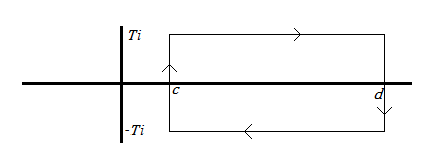
\includegraphics{analytic-chapters/dir-c1.png}
\end{figure}

Hence,
\begin{align*}
\ab{\int_{c-iT}^{c+iT}y^s\frac{ds}{s}}
&=\ab{\int_{c+iT}^{d+iT} y^s\frac{ds}{s}+\int_{d-iT}^{c-iT} y^s\frac{ds}{s}+\int_{d+iT}^{d-iT} y^s\frac{ds}{s}}\\
&\le 2\int_c^d y^{\si}\frac{d\si}{T}+\ab{\int_{d+iT}^{d-iT} y^s\frac{ds}{s}}.
\end{align*}
Note that the last integral goes to 0 as $d\to \iy$, because $|y^s|=|y^d|\to 0$. Hence, taking $d\to \iy$ gives
\[
\ab{\int_{c-iT}^{c+iT}y^s\frac{ds}{s}}
\le 2\int_c^{\iy} \frac{y^{\si}}{T}\,d\si=-\frac{2y^c}{T\ln y}=\frac{2y^c}{T|\ln y|}.
\]
This gives $\ab{\rc{2\pi i}\int_{c-iT}^{c+iT} y^s\frac{ds}{s}}\le \frac{y^c}{\pi T}{|\ln y|}$.

%Now we show the bound $\ab{\rc{2\pi i}\int_{c-iT}^{c+iT} y^s\frac{ds}{s}}\le \frac{y^c}{2}$, for any $y$.
By Cauchy's theorem applied to the smaller segment bounded by $\Re s=c$ and the circle with radius $R=\sqrt{c^2+T^2}$,  \fixme{(picture)} we have
\begin{align*}
%\int_{c-iT}^{c+iT} y^s\frac{ds}{s}+\int_C \frac{y^s}\frac{ds}{s}&=0\\
\ab{\int_{c-iT}^{c+iT} y^s\frac{ds}{s}}
&= \ab{\int_C y^s\frac{ds}{s}}\\
&\le \pi R\frac{y^{c}}{R}=\pi y^c,
\end{align*}
since $y<1$ and $\Re s>c$ on the arc. Hence $\ab{\rc{2\pi i}\int_{c-iT}^{c+iT} y^s\frac{ds}{s}}\le \frac{y^c}2$.\\

For $y>1$, take $d<0$. Note $\frac{y^s}{s}$ is analytic in the region below except for a simple pole at 0 with residue 1 (since $y^s=1$ when $s=0$). Hence by Cauchy's Theorem,
\[
\int_{c-iT}^{c+iT} y^s\frac{ds}{s}+\int_{c+iT}^{d+iT} y^s\frac{ds}{s}+\int_{d+iT}^{d-iT} y^s\frac{ds}{s}+\int_{d-iT}^{c-iT} y^s\frac{ds}{s}=2\pi i.
\]

\fixme{[INSERT PICCY]}

Then 
\begin{align*}
\ab{\int_{c-iT}^{c+iT}y^s\frac{ds}{s}-1}
&=\ab{\int_{c+iT}^{d+iT} y^s\frac{ds}{s}+\int_{d-iT}^{c-iT} y^s\frac{ds}{s}+\int_{d+iT}^{d-iT} y^s\frac{ds}{s}}\\
&\le 2\int_d^c y^{\si}\frac{d\si}{T}+\ab{\int_{d+iT}^{d-iT} y^s\frac{ds}{s}}.
\end{align*}
The last term goes to 0 as $d\to -\iy$, so the same argument applies as in the first part to show $\ab{\rc{2\pi i} \int_{c-iT}^{c+iT}y^s\frac{ds}{s}-1}\le \frac{y^c}{\pi T\ln y}$.

By Cauchy's theorem applied to the larger segment bounded by $\Re s=c$ and the circle with radius $R=\sqrt{c^2+T^2}$, \fixme{(picture)} we have
\begin{align*}
\int_{c-iT}^{c+iT} y^s\frac{ds}{s}+\int_C y^s\frac{ds}{s}&=2\pi i\\
\ab{\int_{c-iT}^{c+iT} y^s\frac{ds}{s}-1}
&\le \ab{\int_C y^s\frac{ds}{s}}\\
&\le 2\pi R\frac{y^{c}}{R}=2\pi y^c,
\end{align*}
since $y>1$ and $\Re s<c$ on the arc. Hence $\ab{\rc{2\pi i}\int_{c-iT}^{c+iT} y^s\frac{ds}{s}}\le y^c$.\\

Proof for $y=1$ omitted.
\end{proof}
\begin{cor}\llabel{sum-coeff-Dir}
The partial sum of the coefficients of a Dirichlet series is given by 
\[
\sum_{n<x} a_n+\frac{a_x}{2}(x\in \N_0)=\rc{2\pi i} \lim_{T\to \iy}\int_{c-iT}^{c+iT} x^s f(s)\frac{ds}{s}.
\]
The error from truncating the integral is
\[
\ab{\pa{\sum_{n<x} a_n+\frac{a_x}{2}(x\in \N_0)}-\pa{\rc{2\pi i} \int_{c-iT}^{c+iT} x^s f(s)\frac{ds}{s}}}\le \sum_{n=1}^{\iy} \pf xn^c a_n\min\pa{1,\rc{T\ab{\ln\pf xn}}}.
\]
\end{cor}


%%%%%%%%%%%%
\chapter{Zeta functions and the prime number theorem}\llabel{zeta-l-pnt}
\index{prime number theorem}
\section{Prime number theorem: Outline}
\begin{df}
Define the prime-counting function
\[
\pi(x)=|\set{p\le x}{p\text{ prime}}|.
\]
\end{df}
Our goal in this chapter is to prove the following famous theorem (in all its error-bounded glory).
\begin{thm}[Prime number theorem]\llabel{pnt}
There is an effective constant $C>0$ such that
\[
\pi(x)=\text{li}(x)+O(xe^{-C\sqrt{\ln x}})
\]
for all $x\ge 1$.
\end{thm}
Here $\Li(x)$ denotes the \textbf{logarithmic integral}
\[
\Li(x)=\int_2^x \frac{dt}{\ln t}.
\]
Note that $\Li(x)= \frac{x}{\ln x}+O\pf{x}{(\ln x)^2}$ as $x\to \iy$, since integration by parts gives
\begin{align}
\nonumber\li(x)&=\int_2^x \frac{dy}{\ln y} +O(1)=\frac{x}{\ln x}+\int_2^x \frac{dy}{(\ln y)^2}+O(1)\\
&=\frac{x}{\ln x}+O\pf{x}{(\ln x)^2}.\llabel{li-ibp}
\end{align}

\subsection{The big picture}

We recommend Andrew Granville's article IV.2 Analytic Number Theory in~\cite{PCTM} for an overview.

How might we guess at the asymptotics for $\pi(x)$? (In particular, why is it closer to $\Li(x)$ than $\fc{x}{\ln x}$?) By studying tables of primes up to 3 million, Gauss hypothesized that the density of primes at around $x$ is around $\rc{\ln x}$, and hence that the number of primes up to $x$ would be the integral $\Li(x)=\int_2^x \frac{dt}{\ln t}$. Making a table of $\pi(x)$ and the difference $\Li(x)-\pi(x)$, we find that the difference is slightly more than on the order of $\sqrt x$, so this seems to be a good estimate.

It is a common theme in analytic number theory to make conjectures about the distribution of primes (or other subsets of interest) by assuming they are randomly distributed according to some probability model. Often a simple model works for simple asymptotics up to $x$, and the model needs to be refined or corrected when dealing with more complicated quantities such as number of primes in a small interval, or spacing between primes.

\begin{mdl}[Gauss-Cram\'er model]
For $n\ge 3$, let $X_n$ be the random variable such that
\begin{align*}
X_n&=1 \text{ with probability }\rc{\ln n}\\
X_n&=0 \text{ with probability }1-\rc{\ln n}.
\end{align*}
Then the sequence $X_n$ behaves similarly to the sequence 
\begin{align*}
a_n&=1 \text{ if $n$ is prime}\\
a_n&=0 \text{ otherwise.}
\end{align*}
\end{mdl}
The Gauss-Cram\'er model exactly predicts $\pi(x)\sim \Li(x)$. The model gives more than just the asymptotics of $\pi(x)$, though, it can also be used to think about primes in short intervals $\pi(x+y)-\pi(x)$. \\

\prbbox{What are the shortcomings of the Gauss-Cram\'er model?}
\vskip0.15in

\subsection{Main steps}
The main steps in the proof are as follows.
\begin{enumerate}
\item When we have a Dirichlet series
\[
F(s)=\sum_{n=0}^{\iy} a_n n^{-s},
\]
we can get estimates for $\sum_{n=0}^N a_n$ by ``plucking out" those coefficients: The equation %using the Mellin transform:
\[
\rc{2\pi i}\lim_{T\to\iy}\int_{c-iT}^{c+iT} y^s\frac{ds}{s}=\begin{cases}
1,&\text{if }y>1\\
\rc 2,&\text{if }y=1\\
0,&\text{if }y<1.
\end{cases}
\]
gives
\[
\rc{2\pi i} \lim_{T\to \iy}\int_{c-iT}^{c+iT} x^s f(s)\frac{ds}{s}=\sum_{n<x} a_n+\frac{a_x}{2}(x\in \N_0).
\]
We use the more precise statement giving error bounds (Corollary~\ref{dirichlet}.\ref{sum-coeff-Dir}).

We want a Dirichlet series where the sum of the first $N$ terms is related to $\pi(N)$.
Let
\[
\ze(s)=\prod_{p\text{ prime}} \rc{1-p^{-s}}=\sum_{n=1}^{\iy}\rc{n^s}.
\]
We consider the function
\[
-\frac{\zeta'(s)}{\zeta(s)}=\sum_{p\text{ prime}} \frac{(\ln p)p^{-s}}{1-p^{-s}}
=\sum_{n=1}^{\iy} \La(n)n^{-s}.
\]
We use this function because $\psi(x):=\sum_{n<x} \La(n)$ gives information on $\pi(x)$, and 
$-\frac{\zeta'}{\zeta}$ continues into a meromorphic function on $\C$ (since $\ze$ does). We now have the estimate
\[
\psi(x)=\rc{2\pi i}\int_{c-iT}^{c+iT} -\frac{\zeta'(s)}{\zeta(s)} x^s\frac{ds}{s}+(\text{error}).
\]
\item We know $\zeta$ has analytic continuation (Theorem~\ref{zeta-continues}). Hence we can move the path of integration to $c<0$. From Cauchy's integral formula, we get extra terms from the horizontal integrals (integrals involving $-\frac{\zeta'}{\zeta}$) and terms $\frac{x^{\rho}}{\rho}$ from Cauchy's integral theorem from the zeros of $\zeta(s)$. {\it This is why we care about its zeros!} Zeros with large real part contribute large error terms.
We will need the following.
\begin{enumerate}
\item
We apply the product development (Theorem~\ref{complex-analysis}.\ref{product-development}) on $\xi(s)=\pi^{-\frac s2}\zeta(s)\Ga\pf s2$ to obtain
\[
\frac{\zeta'(s)}{\zeta(s)}=\sum_{\rh\text{ zero of }\zeta}\pa{\rc{s-\rh}+\rc{\rh}}+\cdots
\]
(Theorem~\ref{xi-product-development}).
%\[
%\frac{\ze'(s)}{\ze(s)}=\sum_{|T-\Im \rh|<1}\rc{s-\rh}+O(\ln T).
%\]
%(See Theorem~\ref{zeta-l-pnt}.\ref{zeta-product-development}).
\item
Using the above equation for $\frac{\zeta'}{\zeta}$, we calculate the asymptotics of $N(T)$, the number of zeros in $\set{\si+it}{(\si,t)\in[0,1]\times[-T,T]}$ (Theorem~\ref{zeta-zeros}).
\item
From (a) to (b) we get a zero-free region for $\ze$ (which includes $\Re s\ge 1$) (Theorems~\ref{weak-zeta-zeros} and \ref{zeta-zero-free}).
\end{enumerate}
From the zero-free region we get a bound for $\sum\frac{x^{\rh}}{\rh}$, as well as the horizontal integrals. 
If the Riemann hypothesis is true, then we can enlarge our zero-free region to $\Re s> \rc2$, which is even better. 
\item Finally we use the estimate for $\psi(x)$ to get an estimate for $\pi(x)$ (Lemma~\ref{partial-sum-pi}).
\end{enumerate}
\index{zeta function}
%\index{zeta function|Riemann}
%\index{zeta function|Hurwitz}
\section{Riemann zeta function}
\begin{df}
The \textbf{Riemann zeta function} is defined by %, the $L$-function with character $\chi$, and the \textbf{Hurwitz zeta function}, are respectively given by
%\begin{align*}
\[
\zeta(s)=\sum_{n=1}^{\iy} \rc{n^s}
%L(s,\chi)&=\sum_{n=1}^{\iy} \frac{\chi(n)}{n^s}\\
%\zeta(s,a)&=\sum_{n=0}^{\iy} \rc{(n+a)^s},&0<a\le 1.
%\end{align*}
\]
when $\Re s>1$. This will be generalized to $L$-functions $L(s,\chi)$ in Definition~\ref{l-func-dirichlet}.\ref{l-func-def}.
\end{df}
%Note that the $L$-function and $\zeta(s,a)$ are generalizations of $\zeta$ in different directions.
%Note
%\[
%L(s,\chi)=k^{-s}\sum_{r=1}^k \chi(r)\zeta\pa{s,\frac rk}.
%\]
By Theorem~\ref{euler-product} and by unique factorization in $\Z$, we can write
\[
\ze(s)=\prod_{p\text{ prime}}\rc{1-p^{-s}}.
\]
By taking the logarithmic derivative, we have %(VALID BY...), we have
\[
-\frac{\zeta'(s)}{\zeta(s)}=\sum_p \frac{d}{ds}\ln(1-p^{-s})
=\sum_p (\ln p)\frac{p^{-s}}{1-p^{-s}}=\sum_p \ln p\sum_{k=1}^{\iy} p^{-ks}.
\]
Interchanging order of summation gives
\begin{equation}\llabel{log-diff-zeta}
-\frac{\zeta'(s)}{\zeta(s)}=\sum_{n=1}^{\iy} \La(n)n^{-s}, \quad \Re s>1,
\end{equation}
where the von Mangoldt function $\La(n)$ is defined as
\[
\La(n)=\begin{cases}
\ln p,&n=p^r,\,p\text{ prime, }r\in \N.\\
0,&\text{else}
\end{cases}
\]

The most important property of $\ze$ is its analytic continuation and functional equation.
\begin{thm}\llabel{zeta-continues}
$\zeta(s)$ can be analytically continued to a meromorphic function with a simple pole at $s=0,1$. %with residue 1. 
It satisfies the functional equation
\[
\zeta(s)=2(2\pi)^{s-1}\Ga(1-s)\sin\pf{\pi s}2 \zeta(1-s).
\]
Letting $\xi(s)=\pi^{-\frac s2}\zeta(s)\Ga\pf s2$, we have\footnote{The factor $\Ga\pf s2$ can be thought of as coming from the infinite place---see Chapter~\ref{l-nf}.}
\[
\xi(s)=\xi(1-s).
\]
Moreover, $\ze(s)$ has zeros $-2\N$ (the trivial zeros); all other zeros are in the critical strip $0\le \Re s\le 1$.
\end{thm}
To prove this, we first need the transformation law for the theta function; we will show the functional equation for $\ze$ by writing it in terms of $\te$. As we will prove a more generalized transformation law, we will postpone the proof for $\te$.
\begin{df}
Define the \textbf{theta function} by
\[
\te(u)=\sum_{n\in \Z}e^{-\pi n^2u},\quad \Re u>0.
\]
\end{df}
\begin{pr}[Transformation law for $\te$]\llabel{theta-law}
For all $u$ with $\Re u>0$,
\[
\te\prc u = u^{\rc2} \te(u).
\]
\end{pr}
This is a special case of Proposition~\ref{l-func-dirichlet}.\ref{theta-transforms}.
\begin{proof}[Proof of Theorem~\ref{zeta-continues}]
We first analytically continue $\zeta$ to $\Re s>0$, show the functional equation is true for $0<\Re s<1$, and use it to establish analytic continuation to $\C$.

Note
\begin{equation}\llabel{continue-zeta-to-0}
\zeta(s)=\rc{s-1}+\sum_{n=1}^{\iy}\ba{
n^{-s}-\int_n^{n+1} x^{-s} \,dx
}
=\rc{s-1}+\sum_{n=1}^{\iy} \int_n^{n+1} (n^{-s}-x^{-s})\,dx
\end{equation}
Since for $n\le x\le n+1$ we have
\begin{align}
\nonumber|n^{-s}-x^{-s}|&=\ab{\int_{n}^x sx^{-s-1}\,dx}
\le|s|n^{-s-1}\\
\llabel{bound-zeta-summands}
\ab{\int_n^{n+1} n^{-s}-x^{-s}\,dx}&\le |s|n^{-s-1},
\end{align}
the sum~(\ref{continue-zeta-to-0}) converges uniformly locally for $\Re s>0$ and extends $\zeta$ to an analytic function for $\Re s>0$.

We claim that
\begin{equation}\llabel{zeta-theta}
2\xi(s)=\int_0^{\iy} (\theta(u)-1)u^{\frac s2} \frac{du}{u},\quad \Re s>1
\end{equation}
%i.e. $\zeta(-2s)$ is the Mellin transform of $\frac{\theta(u)-1}2$.
Indeed, we have
\begin{align*}
\int_0^{\iy} (\theta(u)-1)u^{\frac s2} \,\frac{du}u
&=\int_0^{\iy} 2\sum_{n=1}^{\iy} e^{-\pi n^2u}u^{\frac s2}\frac{du}u\\
&=2\sum_{n=1}^{\iy} \int_0^{\iy} e^{-\pi n^2u}u^{\frac{s}2}\,\frac{du}u\\%absolute convergence?
&=2\sum_{n=1}^{\iy} \int_0^{\iy} e^{-u} \pf{u}{\pi n^2}^{\frac s2}\,\frac{du}u&u\mapsfrom \frac{u}{\pi n^2}\\
&=2\pi^{-\frac s2}\pa{\sum_{n=1}^{\iy} \rc{n^s}}\pa{\int_0^{\iy} e^{-u} u^{\frac s2}\,\frac{du}u}\\
&=2\pi^{-\frac s2} \zeta(s)\Ga\pf{s}2=2\xi(s).
\end{align*}
The theta transformation law~\ref{theta-law} give that for $\Re s>1$,
\begin{align*}
2\xi(s)&=\int_0^1 (\theta(u)-1)u^{\frac s2}\frac{du}u
+\int_1^{\iy} (\theta(u)-1)u^{\frac s2} \frac{du}{u}\\
&=%-\frac{2}{s}+
\int_1^{\iy} \pa{\theta\prc u-1}u^{\frac s2} \frac{du}u +\int_1^{\iy} (\theta(u)-1)u^{\frac s2}\frac{du}u&u\mapsfrom \rc u\\
&=\int_1^{\iy}\pa{u^{-\rc2}\te\prc u-1} u^{\frac{1-s}2}\frac{du}u+\int_1^{\iy}(u^{\fc{1-s}2}-u^{-\fc{s}2})\fc{du}u
+\int_1^{\iy} (\theta(u)-1)u^{\frac s2}\frac{du}u\\
&=-\frac{2}{s}-\frac{2}{1-s}+\int_1^{\iy} (\theta(u)-1)u^{\frac{1-s}2}\frac{du}u+\int_1^{\iy}(\te(u)-1) u^{\frac s2}\frac{du}u.
\end{align*}
The last expression converges for all $\Re s>0$, so in fact equals $2\ze(s)$ for all $\Re s>0$ by uniqueness of analytic continuation. Since the last expression is symmetric under $1-s\mapsto s$, the functional equation for $\xi$ follows.

%To get the functional equation for $\ze$, note
The functional equation for $\xi$ gives
\begin{align*}
\ze(s)&=\pi^{\fc s2} \Ga\pf s2^{-1}\pi^{-\fc{1-s}2} \Ga\pf{1-s}2\ze(1-s)\\
&=\pi^{s-\rc2} \frac{\Ga\pf{1-s}2}{\Ga\pf{s}2}\ze(1-s)\\
&=\pi^{s-\rc2}\Ga\pf{1-s}2 \Ga\pa{1-\fc s2} \frac{\sin\pf{\pi s}2}{\pi}\ze(1-s)&\text{by Proposition~\ref{complex-analysis}.\ref{gamma-facts}(5)}\\
&=2(2\pi)^{s-1}\sin\pf{\pi s}2\Ga(1-s)\ze(1-s)&\text{by Proposition~\ref{complex-analysis}.\ref{gamma-facts}(6)}
\end{align*}

Finally, the statement about zeros follows from the fact that $\ze$ has no zeros with $\Re s>1$ (as $\fc{\ze'}{\ze}$ is holomorphic there) and the functional equation, noting $\sin\pf{\pi s}{2}=0$ exactly when $s$ is an even integer, with the zero at $s=0$ cancelled by the pole at 1 of $\ze$.
\end{proof}
\begin{thm}[Product development of $\xi$]\llabel{xi-product-development}
The function $(s^2-s)\xi(s)$ is entire of order 1, and $\xi(s)$ has the product expansion
\[
\xi(s)=\frac{e^{A+Bs}}{s^2-s}\prod_{\rho\text{ zero of }\ze} \pa{1-\frac s{\rh}}e^{\frac s{\rh}}.
\]
Then $\frac{\zeta'}{\zeta}(s)$ has the partial-fraction expansion
\[
\frac{\zeta'}{\zeta}(s)=B-\rc{s-1}+\rc{2}\ln(\pi) -\rc2\frac{\Ga'}{\Ga}\pa{\frac s2+1}+\sum_{\rh\text{ nontrivial zero of }\zeta}\pa{\rc{s-\rh}+\rc{\rh}}.
\]
\end{thm}
From now on, unless otherwise specified, when we say zero of $\ze$ we mean {\it nontrivial} zero.
\begin{proof}
Note $(s^2-s)\xi(s)$ is entire because $\xi$ only has 2 simple poles at $0,1$. To show it has order 1 we need two inequalities.\\

\noindent \underline{Step 1:} There is no constant $C$ so that $(s^2-s)\xi(s)\precsim e^{C|s|}$: Indeed, for real $s$ and any constant $C$, by Stirling's approximation~\ref{complex-analysis}.\ref{stirling} we have
\begin{align*}
(s^2-s)\xi(s)&=(s^2-s)\pi^{-\frac s2}\Ga\pf s2\ze(s)\\
&\succsim s^{-\rc 2}\pf{s}{2e\pi}^{\frac s2}
\succsim e^{Cs}.
\end{align*}
\noindent\underline{Step 2:} There is a constant $C$ so that $(s^2-s)\xi(s)\precsim e^{C|s|\ln|s|}$: $e^{|s|\ln|s|}\ge1$ for all $s$ so it suffices to prove this for sufficiently large $s$. By the integral and sum formulas for $\Ga$ and $\xi$, and the fact that $|x^s|=|x^{\Re s}|$, we have
\[
|\xi(\si+ti)|\le \pi^{-\frac{\si}{2}}\Ga\pf{\si}{2}\ze(\si),\quad \si>1.
\]
By symmetry of $\xi$ is suffices to consider $\si\ge \rc2$. (``Nudging" $|s|$ in $e^{C|s|\ln|s|}$ by a constant changes it by at most a constant factor.)
Consider 2 cases.
\begin{enumerate}
\item
$\si>2$: Then $\pi^{-\frac{\si}{2}}<1$ and $\ze(\si)<\ze(2)$ so by Stirling's approximation~\ref{complex-analysis}.\ref{stirling},
\[
|\xi(\si+ti)|\precsim
\Ga\pf{\si}2
%\precsim %\pf{\si}{2}^{\frac{\si}2-\rc 2}e^{-\frac{\si}{2}}
=e^{|(\ln\Ga)(\si)|}=e^{\pa{\frac{\si}2-1}\ln\frac{\si}2-\frac{\si}2+O(1)}
\]
from which the result follows.
\item
$\frac12\le \si\le 2$: From~(\ref{bound-zeta-summands}), we have for $s$ bounded away from 1,
\[
\zeta(s)\le O(1)+|s| \sum_{n=1}^{\iy} n^{-\frac 32}=O(|s|).
\]
This time $\Ga\pf{\si}{2}=O(1)$ so
\[
|(s^2-s)\xi(s)|\le \ab{
s^2\pi^{-\frac{\si}2}\zeta(s)\Ga\pf{\si}2}
=O(|s|^3)\precsim e^{C|s|\ln|s|}.
\]
\end{enumerate}
This shows $(s^2-s)\xi(s)$ has order 1.\\

\noindent\underline{Step 3:} By the product development~\ref{complex-analysis}.\ref{product-development}, noting the the zeros of $(s^2-s)\xi$ are the nontrivial zeros of $\ze$ (since $\Ga$ has no zeros and trivial zeros of $\ze$ come from the poles of $\Ga$ in the definition of $\xi$), we get
\[
(s^2-s)\xi(s)=e^{A+Bs}\prod_{\rh\text{ zero of }\zeta}\pa{1-\frac{s}{\rh}}e^{\frac s{\rh}}.
\]
Dividing by $s^2-s$ and log-differentiating gives
\[
\frac{\xi'}{\xi}(s)=B-\rc{s}-\rc{s-1}+\sum_{\rh} \pa{\rc{s-\rh}+\rc{\rh}}.
\]
Since $\ze(s)=\pi^{\frac s2}\Ga\pf{s}2^{-1}\xi(s)$, we get
\begin{align*}
\frac{\ze'}{\ze}(s)&=\rc{2}\ln\pi +\rc2\frac{\Ga'}{\Ga}\pa{\fc s2}+B-\rc{s}-\rc{s-1}+\sum_{\rh} \pa{\rc{s-\rh}+\rc{\rh}}\\
&=\rc{2}\ln\pi +\rc2\frac{\Ga'}{\Ga}\pa{\fc s2+1}+B-\rc{s-1}+\sum_{\rh} \pa{\rc{s-\rh}+\rc{\rh}},&\Ga(z)=\fc{\Ga(z+1)}{z}.\qedhere
\end{align*}
\end{proof}
\section{Zeros of zeta}
Note that from the function equation, $\ze(s)$ has simple zeros at $-2\N$. We call these trivial zeros. More importantly for us are the zeros with real part in $[0,1]$.

Denote by $N(T)$ be the number of zeros of $\zeta$ in $\set{\si+it}{(\si,t)\in [0,1]\times [-T,T]}$, counting multiplicity. We first give asymptotics on the vertical distribution of zeros of $\zeta$ (von Mangoldt's formula, Theorem~\ref{zeta-zeros}), then give a zero-free region for $\zeta$ (Theorem~\ref{zeta-zero-free}).
\begin{lem}\llabel{weak-zeta-zeros}
Define $\cal L(t)=\ln (|t|+2)$. 
For $s=\si+it$ with $\si\in [-1,2]$, we have\footnote{Note $\rc{s-1}=O(1)$ when $s$ is bounded away from 1.}
\begin{align}
\llabel{weak-zeta-zeros-eq1}
\frac{\zeta'(s)}{\zeta(s)}
&={\color{gray}-\rc{s-1}}
+\sum_{\rh}\pa{\rc{s-\rh}+\rc{\rh}}+O(\cal L)\\
\nonumber
&={\color{gray}-\rc{s-1}}
+\sum_{|\Im(s-\rh)|<1} \rc{s-\rh} +O(\cal L).
\end{align}
Moreover, there are $O(\cal L)$ zeros $\rh$ with $|\Im(s-\rh)|<1$, i.e. the number of zeros with imaginary part in $[t,t+1]$ is $O(\ln t)$, as $t\to \iy$.
\end{lem}
Note this gives $N(T)=O(T\ln T)$. The next theorem will give an improvement of this estimate.
\begin{proof}
Our strategy is this: at a point where we know $\frac{\ze'}{\ze}$ is bounded ($s=2+it$), we use Theorem~\ref{xi-product-development} to get information on how many zeros of $\zeta$ can be close to $s$. Then we use compare $\frac{\ze'}{\ze}(\si+it)$ with $\frac{\ze'}{\ze}(2+it)$ to get the general estimate.\\

\noindent\underline{Step 1:}
Theorem~\ref{xi-product-development} gives us
\begin{equation}\llabel{zeta2-zero-sum}
\frac{\zeta'(s)}{\zeta(s)}=-\rc{s-1}+
\underbrace{B+\rc2\ln\pi}_{O(1)}
-
\rc2\underbrace{\frac{\Ga'}{\Ga}\pa{%\frac{\si}2+1+i\frac t2}
\frac s2+1}}_{(A)}+
\underbrace{\sum_{\rh} \pa{\rc{%\si+it
s-\rh}+\rc{\rh}}}_{(B)}.
\end{equation}
From Stirling's approximation~\ref{complex-analysis}.\ref{stirling}, (A) equals
\begin{equation}\llabel{gamma2-estimate}
%\underbrace{
\ln\ab{\frac{\si}{2}+1+i\frac t2}%}_{O(1+\ln |t|)}
+O(1)=
%\underbrace{\frac{1}{2\ab{\frac{\si}{2}+1+i\frac t2}}}_{O(1)}
%+O\pa{\ab{\frac{\si}{2}+1+i\frac t2}^{-2}}=
%O(\ln |t|).
O(\cal L)
\end{equation}
These two equations show~(\ref{weak-zeta-zeros-eq1}).

Now suppose $s=2+it$. %Theorem~\ref{xi-product-development} says
Note that
\[
\ab{\frac{\ze'(2+it)}{\ze(2+it)}}
=\ab{\sum_{n=1}^{\iy} \La(n)n^{-2-it}}
\le \ab{\sum_{n=1}^{\iy} (\ln n)n^{-2}}<\iy,
\]
so the LHS of~(\ref{zeta2-zero-sum}) is $O(1)$.
%%%%%%
%Now we estimate (B) by truncating the sum.
Hence~(\ref{zeta2-zero-sum}) becomes
\begin{equation}\llabel{zeta2-zero-sum2}
O(\cal L)=\sum_{\rh} \pa{\rc{%\si+it
s-\rh}+\rc{\rh}}.
\end{equation}
%Note
%\[
%\Re\pa{\rc{2+it-\rh}+\rc{\rh}}=\Re\pa{
%\frac{(2+\Re \rh)-(t-\Im \rh)i}{(2-\Re \rh)^2+(t-\Im\rh)^2}
%}
%\ge\rc{4+(t-\Im \rh)^2}
%\]
%since $0\le \Re \rh\le 1$.
We estimate the terms with $|\Im(s-\rh)|<1$ by a constant to show that there aren't too many of them.
From~(\ref{zeta2-zero-sum2}) and~(\ref{gamma2-estimate}),
\begin{align}
%O(\ln |t|) &\ge \Re\sum_{|\Im(s-\rh)|<1}\pa{\rc{2+it-\rh}+\rc{\rh}}\\
%%&\ge \Re\sum_{
%%%{\footnotesize\begin{array}{c}
%%%\rh\text{ zero}\\
%%|\Im(s-\rh)|<1%\end{array}}}
%%}\frac{(2+\Re \rh)-(t-\Im \rh)i}{(2-\Re \rh)^2+(t-\Im\rh)^2}\\
%&=\sum_{|\Im(s-\rh)|<1}\rc{4+(t-\Im \rh)^2}\\
%&\ge \rc 5 |\set{\rh}{|\Im(s-\rh)|<1}|.
%
\nonumber
O(\cal L) &= \Re\sum_{\rh}\pa{\rc{2+it-\rh}+\rc{\rh}}\\
\nonumber
&\ge
\Re\sum_{\rh}\pa{
\frac{(2-\Re \rh)-(t-\Im \rh)i}{(2-\Re \rh)^2+(t-\Im\rh)^2}
}&\text{since }\Re \prc{\rh}>0\\
\nonumber
&\ge\sum_{\rh} \rc{4+(t-\Im \rh)^2}&\text{since $0\le \Re \rh\le 1$}\\
\llabel{zero-olnt}
&\ge \rc 5 |\set{\rh}{|\Im(s-\rh)|<1}|+\rc5 \sum_{|\Im(s-\rh)|\ge 1}\rc{(t-\Im \rh)^2}.
\end{align}
This proves the second part of the lemma.\\
%%We similarly consider the sum for $|\Im(s-\rh)|>1$:
%%\begin{align}
%%\llabel{olntge}
%%O(\ln|t|)
%%&\ge\sum_{|\Im(s-\rh)|\ge 1}\pa{\rc{2+it-\rh}+\rc{\rh}}\\
%%\nonumber&=\sum_{|\Im(s-\rh)|<1}\rc{4+(t-\Im \rh)^2}\\
%%\nonumber&\ge \rc5 \sum_{|\Im(s-\rh)|<1}\rc{(t-\Im \rh)^2}
%%\end{align}
%Now from~(\ref{zeta2-zero-sum}),
%\begin{align*}
%\ab{\frac{\zeta'(2+it)}{\zeta(2+it)}}
%%O(\ln|t|)
%&=\sum_{|\Im(s-\rh)|<1}\rc{s-\rh}+
%\underbrace{\sum_{|\Im(s-\rh)|<1}\rc{\rh}}_{O(\ln|t|)}
%+
%\underbrace{\sum_{|\Im(s-\rh)|\ge 1}\pa{\rc{2+it-\rh}+\rc{\rh}}}_{O(\ln|t|)}
%%&=O(\ln|t|)+\sum_{|\Im(s-\rh)|<1}\rc{s-\rh}+O(\ln|t|)+O(\ln|t|),
%\end{align*}
%as needed. (The first $O(\ln|t|)$ is because there are $O(\ln|t|)$ terms in the sum and each is at most 1 in absolute value.)\\

\noindent\underline{Step 2:} Now we consider general $s=\si+it$, by comparing it to $2+it$. We have by~(\ref{zeta2-zero-sum}) and~(\ref{gamma2-estimate}) that
\begin{align*}
&\quad \frac{\zeta'}{\zeta}(s)-\underbrace{\frac{\ze'}{\ze}(2+it)}_{O(1)}\\
&=-\rc{s-1}+O(1)+\underbrace{\rc2\pa{\ln\ab{\frac{\si}2+1+\frac t2i}-
\ln\ab{2+\frac t2i}}}_{O(1)}+\sum_{\rh} \pa{\rc{s-\rh}-\rc{2+it-\rh}}\\
&=-\rc{s-1}+O(1)+
\sum_{|\Im(s-\rh)|<1}\rc{s-\rh}-\underbrace{\sum_{|\Im(s-\rh)|<1}\rc{2+it-\rh}}_{O(\cal L)}+
\underbrace{\sum_{|\Im(s-\rh)|\ge1}\frac{(2-\si)}{(s-\rh)(2+it-\rh)}}_{O(\cal L)}.
\end{align*}
The first $O(\cal L)$ is because there are at most $O(\cal L)$ terms and each term is at most 1 in absolute value; the second is from
\[
\sum_{|\Im(s-\rh)|\ge1}\frac{2-\si}{(s-\rh)(2+it-\rh)}=O\pa{\sum_{|\Im(s-\rh)|\ge1}\frac{1}{\Im(s-\rh)^2}}=O(\cal L);
\]
the first equality is from $2-\si=O(1)$ and $\Im(s-\rh)=\Im(2+it-\rh)$; the second is by~(\ref{zero-olnt}).
\end{proof}
\index{von Mangoldt's Theorem}
\begin{thm}[von Mangoldt]\llabel{zeta-zeros}($*$) 
As $T\to \iy$,
\[
N(T)=\frac{T}{\pi}\ln\pf{T}{2\pi}-\frac{T}{\pi}+O(\ln T).
\]
\end{thm}
\begin{proof}
As $\zeta$ has only a countable number of zeros, we may assume $T$ is not the imaginary part of any zero.

Let
\[
\cal R=\set{\si+it}{(s,t)\in [-1,2]\times [-T,T]}
\]
and let $C$ be the boundary of $\cal R$. \fixme{(PICTURE)}
%Since $\Ga(\ol s)=\ol{\Ga(s)}$, the zeros of $\Ga$ are symmetric across the real axis. 
From $\xi(s)=\pi^{-\frac s2}\zeta(s)\Ga\pf s2$, we see that $\xi$ has the same zeros as $\zeta$ in this region, and simple poles at $0$ and $1$. %Now $\Ga$ has $2N(T)$ zeros (note it has no zeros on the real axis)
%and $2$ poles in $\cal R$, namely $0$ and $1$. 
Hence by Cauchy's residue formula~\ref{complex-analysis}.\ref{residue},
\[
\rc{2\pi i}\oint_{C} \frac{\xi'(s)}{\xi(s)} ds=2N(T)-2.
\]
Noting that $\xi(\ol{s})=\ol{\xi(s)}$ and $\xi(s)=\xi(1-s)$, changes of variable show that the integral on each of the sections of $C$ between $2$, $\rc 2+iT$, $-1$, and $\rc 2-iT$ are the same.\footnote{We used $\xi$ because its symmetry allows us to do this.} Let $C'$ be the part from $1$ to $\rc 2+iT$. Thus 
%(using $\pa{\prod_{k=1}^n f_k}'=\sum_{k=1}^n \frac{f_k'}{f_k}$), 
the above equals
\begin{align*}
\frac2{\pi i}\int_{C'} \frac{\xi'(s)}{\xi(s)} ds
&=\frac2{\pi i}
\int_{C'} -\frac{\ln \pi}{2}+\frac{\zeta'(s)}{\zeta(s)}+\frac{\pa{\Ga\pf{s}{2}}'}{\Ga\pf s2}\,ds&\frac{\pa{\prod_{k=1}^n f_k}'}{\prod_{k=1}^n f_k}=\sum_{k=1}^n \frac{f_k'}{f_k}\\
&=\frac2{\pi}\Im
\int_{C'} -\frac{\ln \pi}{2}+\frac{\zeta'(s)}{\zeta(s)}+\frac{\pa{\Ga\pf{s}{2}}'}{\Ga\pf s2}\,ds
&\text{(expression is real)}.
\end{align*}
We break this up into 3 integrals and estimate each part separately.
\begin{enumerate}
\item $\Im\int_{C'}-\frac{\ln \pi}{2}\,ds=-\frac{T}{2}\ln \pi$.
\item Using the estimate for $\frac{\zeta'}{\zeta}$ in Lemma~\ref{weak-zeta-zeros},  we evaluate the second integral. Note that $\ln\zeta$ is defined for $\Re s> 1$ and is uniformly bounded for $\Re s=2$:
\begin{align*}
(\ln\zeta)(s)&=\sum_{p\text{ prime}} \ln(1-p^{-s}) \\
|(\ln\zeta)(2+it)|&\le\sum_{p\text{ prime}} 2p^{-2}.
\end{align*}
(Just bound $\ln$ linearly near 1, or expand in Taylor series.)  
Note $\ln(x-\rh)$ is well-defined on $C'$ for any $\rh$. Hence by Theorem~\ref{weak-zeta-zeros},
\begin{align*}
\Im\int_{C'}\frac{\zeta'}{\zeta}(s)\,ds
&=(\Im(\ln\zeta)(2+iT)-{\Im(\ln\zeta)(2)})+\int_{2+iT}^{\rc 2+iT} \frac{\zeta'}{\zeta}(s)\,ds\\
&=O(1)+\int_{2+iT}^{\rc 2+iT} \Im\pa{\sum_{|\Im(s-\rh)|<1}\rc{s-\rh}}+O(\ln T)\,ds\\
&=O(\ln T)+\sum_{|\Im(s-\rh)|<1}\Im(\ln(x-\rh))|^{\rc2+Ti}_{2+Ti}\\
&\le O(\ln T)+2\pi O(\ln T)
\end{align*}
since there are at most $\ln T$ terms in the sum.
\item We estimate the last integral using Stirling's formula~\ref{complex-analysis}.\ref{stirling}. (Note that $\ln\Ga$ is well-defined for $s\in C'$.)
\begin{align*}
\int_{C'}\frac{\pa{\Ga\pf s2}'}{\Ga\pf s2}
&=\ba{\Im(\ln\Ga)\pf s2}^{\rc 2+Ti}_2\\
&=\Im(\ln \Ga)\pa{\frac 14+\frac{T}{2}i}\\
&=\Im\ba{\pa{-\rc 4+\frac T2i}\ln\pa{\rc 4+\frac T2i}-\pa{\rc 4+\frac T2i}+O(1)}\\%&\text{by Theorem~\ref{complex-analysis}.\ref{stirling}}\\
&=\frac T2\ln\pf T2-\frac T2+O(1).&\qedhere
\end{align*}
\end{enumerate}
Now put everything together to get
\begin{align*}
N(T)-2&=\frac{2}{\pi}\pa{-\frac T2\ln \pi+O(\ln T)+\pa{\frac T2\ln\pf T2-\frac T2+O(1)}}\\
N(T)&=\frac{T}{\pi}\ln\pf{T}{2\pi}-\frac{T}{\pi}+O(\ln T).
\end{align*}
\end{proof}
\begin{thm}[Zero-free region for $\zeta$]\llabel{zeta-zero-free}
There are no zeros of $\zeta$ with $\Re s\ge 1$. Moreover, there is a constant $c>0$ such that for $|t|>2$, every zero $\si+it$ satisfies
\[
\si<1-\frac{c}{\ln|t|}.
\]
\end{thm}
\fixme{PICTURE!}
\begin{proof}
%(The proof of the first statement will give us motivation for the second.)
%We know that $\frac{\zeta'}{\zeta}$ has no pole for $\Re s>1$, and hence $\zeta$ has no zero for $\Re s>1$. Thus for the first part it suffices to prove that no zero has real part 1.
We already noted $\ze$ has no zero for $\Re s>1$ (Theorem~\ref{zeta-continues}), so for the first part it suffices to prove that no zero has real part 1.

If $\zeta$ had a zero $1+it$, then $\frac{\zeta'}{\zeta}$ would have a pole of positive residue at $1+it$. For $s=\si+it$, $\si>1$ we have $-\frac{\zeta'}{\zeta}(s)=\sum_{n=1}^{\iy} \frac{\La(n)}{n^s}$, so this means that as $\si\to 1^+$,
many of the important terms would have $n^{-it}$ ``close" to $-1$, to make it blow up in the negative direction. For those terms, we have $n^{-2it}$ ``close" to $1$. This would force $-\frac{\zeta'}{\zeta}(\si+2ti)$ to have a pole of positive residue at $1+2ti$, i.e $\zeta$ to have a pole at $1+2ti$, contradicting the fact that it is analytic there.

We now make this idea precise. What we want is an inequality between some function of an angle and its double, so that if one is small it forces the other to be large. So we consider
\[
0\le 2(1+\cos\theta)^2=3+4\cos \theta +\cos 2\theta.
\]
This gives
\[
0\le 3+4\Re(n^{-it})+\Re(n^{-2it}).
\]
Multiplying by $\La(n)n^{-\si}$ and summing, we get
\begin{equation}\llabel{zero-free-zeta-inequality}
0\le 3\pa{-\frac{\ze'}{\ze}(\si)} 
+4\Re\pa{-\frac{\ze'}{\ze}(\si+ti)}
+\Re\pa{-\frac{\ze'}{\ze}(\si+2ti)},\quad\si>1.
\end{equation}
Letting $r$ be the degree of the zero at $1+ti$, we have by Lemma~\ref{weak-zeta-zeros}
\[
0\le\pa{\frac{3}{\si-1}+O(1)}
-\pa{\frac{4r}{\si-1}+O(\cal L)}
+\Re\pa{-\frac{\ze'}{\ze}(\si+2ti)}\text{ as }\si\to 1^+.
\]
If $r\ge 1$, then this gives $-\frac{\ze'}{\ze}(\si+2ti)\to \iy$ as $\si\to 1^+$, contradiction. Hence $r=0$; $1+it$ is not a zero.

For the second statement, we have to use the partial fraction decomposition~\ref{xi-product-development}.
Suppose $\rh=(1-\de)+it$ is a zero. By Lemma~\ref{weak-zeta-zeros}, we have
\[
-\frac{\zeta'(s)}{\zeta(s)} = O(\ln|t|) -\sum_{\rh}\pa{\rc{s-\rh}+\rc{\rh}}\le O(\ln|t|)-\rc{s-\rh}.
\]
%(All terms in the last sum are positive.)
Then
\begin{align*}
-\Re\frac{\zeta'}{\ze}(\si+ti)&\le O(\ln|t|)-\frac{1}{\si+\de-1}\\
-\Re\frac{\zeta'}{\ze}(\si+2ti)&\le O(\ln|2t|)=O(\ln |t|).
\end{align*}
For $\si>1$, plugging this into~(\ref{zero-free-zeta-inequality}) gives
\begin{align*}
0&\le \frac{3}{\si-1}+O(\ln|t|)-\frac{4}{\si+\de-1}\\
\implies \frac{4}{\si+\de-1}&<\frac{3}{\si-1}+C_1\ln|t|
\end{align*}
for some $C_1$.
Now take $\si=1+4\de$ to get
\[
\frac{4}{5\de}<\frac{3}{4\de}+C_1\ln|t|,
\]
giving
\[
\de>\frac{1}{20C_1\ln|t|}
\]
as needed.
\end{proof}
\section{Prime number theorem: proof}
Now we gather everything together to prove the prime number theorem. We first show the following.
\index{von Mangoldt's formula}
\begin{thm}[von Mangoldt's formula]\llabel{von-Mangoldt-formula}
For an integer $x>2$ and $x\ge T$,
\begin{equation}\llabel{v-M-f}
\psi(x)= x-\sum_{|\Im(\rh)|<T}\frac{x^{\rh}}{\rh}
+O\pa{
\frac{x(\ln x)^2}{T}%+
%\frac{x(\ln T)^2}{T}+\ln x
}.
\end{equation}
\end{thm}
\begin{proof}
\noindent{\underline{Step 1:}} We estimate $\psi(x)$ using Theorem~\ref{dirichlet}.\ref{sum-coeff-Dir}. Suppose $x$ is an integer; the theorem gives
\begin{align*}
\ab{\psi(x)-\pa{
\int_{c-iT}^{c+iT} x^s\pa{-\fc{\ze'}{\ze}(s)\frac{ds}s
}}}&\le
\La(x)+
\sum_{n\ge 1,\,n\ne x} \pf xn^c\La(n)\rc{T\ab{\ln\pf xn}}\\
&\le 
\ln(x)+\sum_{n\ge 1,\,n\ne x}\pf xn^c\fc{\ln(n)}{T\ab{\ln\pf xn}}.
\end{align*}
%Assume $x$ is a large integer (i.e. bounded away from 1) and 
Take
\[
c=1+\rc{\ln x}.
\]
Note that this makes $x^c=ex=O(x)$. 
To estimate the sum we split it into several parts.
\begin{enumerate}
\item
$1\le n< \frac{x}{e}$: We have
\begin{align*}
\sum_{1\le n<\frac xe} \pf xn^c \frac{\ln n}{T\ab{\ln\pf xn}}
&\precsim \frac{x\ln x}{T}\sum_{1\le n<x}\rc{n}\\
&\sim \frac{x(\ln x)^2}{T}.
\end{align*}
\item
$\frac xe\le n< ex$: We have
\begin{align*}
\sum_{\frac xe\le n<ex,\,n\ne x}\pf xn^c \ln n\frac{1}{T\ab{\ln\pf xn}}
&\precsim \sum_{\frac xe\le n<ex,\,n\ne x} \cancel{e^{1+\rc{\ln x}}} \frac{\ln n}{T\ab{\ln\pf xn}}\\
&\precsim \rc{T}\sum_{\frac xe\le n<ex,\,n\ne x}\frac{\ln x}{\ab{1-\frac xn}}&\text{ using $\ln x\sim x-1$ when $x\approx 1$}\\
&\precsim \frac{x\ln x}{T}\sum_{\frac xe\le n<ex,n\ne x}\frac{1}{|n-x|}\\
&\precsim\frac{x\ln x}{T}\sum_{1\le n< (e-1)x}\frac{1}{n}\\
&\sim\frac{x(\ln x)^2}{T}.
\end{align*}
\item $n\ge ex$: We have
\begin{align*}
\sum_{n\ge ex} \pf xn^c \frac{\ln n}{T}&<\frac{x}{T}\int_{ex-1}^{\iy} \frac{\ln y}{y^c}\,dy&\frac{\ln y}{y^c}\text{ decreasing for }y>e\\
&=\frac xT\ba{\frac{-y^{-c+1}\ln y}{c-1}-\frac{y^{-c+1}}{(c-1)^2}}^{\iy}_{ex-1}\\
&\sim \frac{x(\ln x)^2}{T}.
\end{align*}
\end{enumerate}
Putting everything together gives
\begin{equation}\llabel{von-M-1}
\ab{\psi(x)-\pa{
\int_{c-iT}^{c+iT} x^s\pa{-\fc{\ze'}{\ze}(s)}\frac{ds}s
}}=O\pa{\frac{x(\ln x)^2}{T}+\ln x}.
\end{equation}

\noindent\underline{Step 2:} We move the line of integration to $\Re s=-1$. Assuming that $T$ is not the imaginary part of any root, by Cauchy's residue theorem~\ref{residue} \fixme{PICTURE}
\[
\int_{c-iT}^{c+iT} \frac{x^s}{s}\frac{\zeta'}{\ze}(s)\,ds
+\underbrace{\int_{c+iT}^{-1+iT} \frac{x^s}{s}\frac{\zeta'}{\ze}(s)\,ds}_{I_{h,1}}
+\underbrace{\int_{-1+iT}^{-1-iT} \frac{x^s}{s}\frac{\zeta'}{\ze}(s)\,ds}_{I_{v}}
+\underbrace{\int_{-1-iT}^{c-iT} \frac{x^s}{s}\frac{\zeta'}{\ze}(s)\,ds}_{I_{h,2}}
=\fc{\ze'}{\ze}(0)-x+\sum_{|\Im\rh|<T}\frac{x^{\rh}}{\rh}.
\]
Here $\fc{x^{\rh}}{\rh}$ are the resuides at the zeros, $-x$ comes from the pole of $\ze$ at 1, and $\fc{\ze'}{\ze}(0)$ comes from the pole of $\rc s$.
Then
\begin{equation}\llabel{von-M-2}
\int_{c-iT}^{c+iT} \frac{x^s}{s}\pa{-\fc{\zeta'}{\ze}(s)}\,ds-x=1+I_{h,1}+I_{h,2}+I_v-\sum_{\Im\rh<T}\frac{x^{\rh}}{\rh}.
\end{equation}
We estimate each summand.
\begin{enumerate}
\item For the horizontal integrals, we use the estimate~\ref{weak-zeta-zeros} to get
\begin{align*}
\ab{\frac{\ze'}{\ze}(s)}&=\ab{\sum_{|\Im(s-\rh)|<1} \rc{s-\rh}}+O(\ln T),\quad s=\si+Ti\\
&\le \sum_{|\Im(s-\rh)|<1}\rc{\Im(s-\rh)}+O(\ln T).
\end{align*}
We would like to bound $\Im(s-\rh)$ away from 0. To do this, note that there are $O(\ln T)$ roots in with $\Im \rh\in [T,T+1]$ by Lemma~\ref{weak-zeta-zeros}. Hence by tweaking $T$ slightly\footnote{Changing $T$ by a constant does not change the error term of~(\ref{v-M-f}); moreover the change in the LHS sum is $O\pa{\fc xT\ln T}=O\pf{x(\ln x)^2}T$.},
we can assume $|\Im(s-\rh)|>\frac{C}{\ln T}$ for all $\rh$. Also by Lemma~\ref{weak-zeta-zeros} there are at most $O(\ln T)$ terms in the sum, so the sum is $O((\ln T)^2)$.
Integrating gives
\begin{align*}
\ab{\int_{c\pm Ti}^{-1\pm Ti} \frac{x^s}{s}\frac{\ze'}{\ze}(s)ds}
%=\int_{c+Ti}^{1+Ti} O(\ln |T|)\,ds
&=O((\ln T)^2)O\prc T\int_{c}^{-1} |x^s|\,ds\\
&=O\pf{(\ln T)^2}{T}O(x)\\%\ab{\ba{\frac{x^s}{\ln x}}^{-1}_c}\\
&=O\pf{x(\ln x)^2}{T}.
\end{align*}
\item For the vertical integral, we use the same estimate, this time noting that $|s-\rh|>1$ for every root $\rh$, since every zero satisfies $\Re \rh>0$. This gives that $\frac{\ze'}{\ze}(s)=O(\ln T )$, and
\begin{align*}
\ab{\int_{-1+Ti}^{-1-Ti}
\frac{x^s}{s}\frac{\ze'}{\ze}(s)\,ds}
&=
O(\ln T )
\int_{-1-Ti}^{-1+Ti} \frac{x^{-1}}{|s|}\,ds
\\
&=
O\pf{\ln T  }{x}
\int_{-T}^{T} \rc{\sqrt{t^2+1}}\,dt\\
&=
O\pf{\ln T  }{x}
\int_{1}^{T+1} \rc{t}\,dt\\
&=
O\pf{(\ln T )^2}{x}=O\pf{x(\ln x)^2}{T}.
\end{align*}
\end{enumerate}
Equations~(\ref{von-M-1}) and~(\ref{von-M-2}) together with the above two estimates give the theorem.
\end{proof}
The final ingredient in the proof of the Prime Number Theorem is the estimate for $\sum_{|\Im(\rh)|<T}\frac{x^{\rh}}{\rh}$ using the zero-free regions for $\ze$ and the estimate for number of zeros of $\ze$.
\begin{proof}[Proof of Theorem~\ref{pnt}]
First, note there can only be a finite number of zeros of $\ze$ with $|\Im(\rh)|<2$, so $\sum_{|\Im(\rh)|<2}\frac{x^{\rh}}{\rh}=O(x^r)$ for some fixed $r<1$.\footnote{In fact, there are zero such zeros.} We estimate $\sum_{2\le |\Im(\rh)|<T}\frac{x^{\rh}}{\rh}$ in two steps.
\begin{enumerate}
\item By Theorem~\ref{zeta-zero-free}, there is $c$ such that for $\rh$ with $2\le |\Im(\rh)|<T$,  
\[
|x^{\rh}|=x^{\Re\rh}\le x^{1-\frac{c}{\ln T}}=xe^{-\frac{c\ln x}{\ln T}}.
\]
\item Using $N(T)=O(T\ln T)$ (Theorem~\ref{zeta-zeros} or the weaker remark after Lemma~\ref{weak-zeta-zeros}),
\begin{align}
\nonumber
\sum_{2\le |\Im(\rh)|<T}\frac{1}{\ab{\rh}}
&\le \sum_{2\le |\Im(\rh)|<T}\frac{1}{\Im(\rh)}\\
\nonumber
&\le \int_2^{T} \frac{dN(t)}{t}&\text{(Riemann-Steltjes integral)}\\
\nonumber
&= \frac{N(T)}{T}-\fc{N(2)}2+\int_2^T \frac{N(t)}{t^2}\,dt
&\text{integration by parts}\\
\nonumber
&=O(\ln T)+\int_2^T O\pf{\ln t}{t}dt\\
\llabel{pnt-step2}
&=O(\ln T)+O((\ln T)^2)=O((\ln T)^2).
\end{align}
\end{enumerate}
Putting these two estimates together,
\begin{align}
\nonumber
\ab{\sum_{|\Im(\rh)|<T}\frac{x^{\rh}}{\rh}}
&\le O(x^r)+\max_{2\le |\Im(\rh)|<T}(|x^{\rh}|)\sum_{2\le |\Im(\rh)|<t}\frac{1}{|\rh|}\\
&\le O(x^r)+O\pa{xe^{-\frac{c\ln x}{\ln T}}(\ln T)^2}.\llabel{xrhorho}
\end{align}
Combining with Theorem~\ref{von-Mangoldt-formula}, and setting $T=e^{\sqrt{\ln x}}$ (so that 
$xe^{-\frac{\ln x}{\ln T}}
=\frac{x}{T}$), we get 
\begin{align*}
|\psi(x)-x|&
= O\pa{
x^r+xe^{-\frac{c\ln x}{\ln T}}(\ln T)^2+\frac{x(\ln x)^2}{T}
}\\
&=O\pa{x^r+xe^{-c\sqrt{\ln x}}\ln x+x(\ln x)^2 e^{-\sqrt{\ln x}}}\\ 
&=O(xe^{-C\sqrt{\ln x}}),%&x^r, x(\ln x)^2 e^{-\sqrt{\ln x}}\prec xe^{-C\sqrt{\ln x}},
\end{align*}
for some $C>0$. This shows 
\begin{equation}\llabel{psi-asymptotic}
\psi(x)=x+O(xe^{-C\sqrt{\ln x}}).
\end{equation}
Finally, we extract the asymptotics of $\pi$ from the following.
\begin{lem}\llabel{partial-sum-pi}
We have the following estimates:
\begin{align*}
\pi(x)&=\frac{\psi(x)}{\ln x}+\int_2^x \psi(y)\frac{dy}{y(\ln y)^2}+O(x^{\rc2}),\\
\psi(x)&=\pi(x)\ln x-\int_2^x \frac{\pi(y)}{y}\,dy +O(x^{\rc2}\ln x).
\end{align*}
\end{lem}
\begin{proof}
Define
\begin{align*}
\ga(n)&=\begin{cases}
1,&n\text{ prime,}\\
0,&n\text{ not prime,}
\end{cases}&
%\quad
%\si'(n)=\begin{cases}
%1,&n\text{ prime power,}\\
%0,&n\text{ not prime power.}
%\end{cases}
\La_1(n)&=\begin{cases}
\ln n,&n\text{ prime,}\\
0,&n\text{ not prime,}
\end{cases}
\end{align*}
and
\[
\psi_1(x)=\sum_{n\le x}\La_1(n).
\]
First note
\begin{align}
\nonumber
|\psi(x)-\psi_1(x)|&=\sum_{2\le r\le \log_2(x)}\sum_{p\mid\,p^r\le x} \ln p\\
\nonumber
&\le \sum_{2\le r\le \log_2(x)} x^{\rc r}\ln x\\
&=O(x^{\rc 2}\ln x+x^{\rc 3}(\ln x)^2)=O(x^{\rc 2}\ln x).
\llabel{psi-psi1-estimate}
\end{align}
%Define
%\[
%\si'(n)
%\]
%Note $\pi(x)=\sum_{n\le x}\si(n)$, and define $\pi'(x)=\sum_{n\le x}\si'(n)$. Note that $\pi(x)-\pi'(x) 

\noindent{\underline{Part 1:}} By partial summation~\ref{arith-f}.\ref{sum-parts} with $u=\La_1$, $U=\psi_1$, and $v=\frac{1}{\ln x}$,
\begin{align*}
\pi(x)&=\sum_{n\le x} \ga(n)\\
&=\sum_{n\le x}\La_1(n) \rc{\ln n}\\
&=\fc{\psi_1(x)}{\ln x} + \int_2^x\psi_1(t)\frac{dt}{t(\ln t)^2}\\
&=\fc{\psi(x)}{\ln x} +O(x^{\rc2}) +\int_2^x\psi(t)\,\fc{dt}{t(\ln t)^2}
+\int_2^x O(t^{-\rc2})\,dt&\by{psi-psi1-estimate}\\
&=\fc{\psi(x)}{\ln x}+\int_2^x\psi(t)\,\fc{dt}{t(\ln t)^2}+O(x^{\rc2}).
\end{align*}
%Combining this with the estimate~(\ref{psi-psi1-estimate}) and noting
%\[
%O\Big(\fc{x^{\rc2}\ln x}{\ln x}+\int_2^x \underbrace{\fc{t^{\rc 2}\ln t}{t(\ln t)}}_{O(t^{-\rc2})}\,dt\Big)=O(x^{\rc2})
%\]
%gives the result.\\

\noindent{\underline{Part 2:}} By partial summation,
\begin{align*}
\psi_1(x)&=\sum_{n\le x} \ga(n)\ln(n)\\
&=\pi(x)\ln x-\int_2^x\frac{\pi(t)}{t} \,dt.
\end{align*}
Combining with~(\ref{psi-psi1-estimate}) gives the result.
\end{proof}
Putting~(\ref{psi-asymptotic}) into Lemma~\ref{partial-sum-pi},
\begin{align*}
\pi(x)&=\fc{x}{\ln x}+O\pf{xe^{-C\sqrt{\ln x}}}{\ln x}+\int_2^x\pa{\frac{1}{(\ln y)^2}+O\pf{e^{-C\sqrt{\ln y}}}{(\ln y)^2}}dy+O(x^{\rc 2})\\
&=\li(x)+O(xe^{-C\sqrt{\ln x}}).&\by{li-ibp}\qedhere
\end{align*}
\end{proof}
\index{Riemann hypothesis}
\section{The Riemann hypothesis}
The following conjecture is worth one million dollars:
\begin{conj}[Riemann hypothesis]
All nontrivial zeros $s$ of $\zeta(s)$ %have real part  $\rc 2$. 
satisfy $\Re s=\rc 2$.
\end{conj}
Note that for no $\ep>0$ has it been proved that all zeros satisfy $\Re s<1-\ep$. Our zero-free region, sadly, has a boundary approaching real part 1 as $t\to \iy$.

One reason that the Riemann hypothesis is important is that it gives a strong error bound in the prime number theorem (as well as many other theorems of analytic number theory).
\begin{thm}
%The Riemann hypothesis is equivalent to the following bound on $\pi(x)$.
Suppose $\rc 2\le \te<1$. The following are equivalent.
\begin{enumerate}
\item
$\zeta(s)$ has no zeros with $\Re s>\te$.
%\item
%$\psi(x)=x+O_{\ep}(x^{\te+\ep})$ for all $\ep>0$.
\item
$\pi(x)=\li(x)+O(x^{\te}\ln x)$.
\item
$\pi(x)=\li(x)+O(x^{\te+\ep})$ for every $\ep>0$, where the constant depends on $\ep$.
\end{enumerate}
In particular, the Riemann hypothesis is equivalent to $\pi(x)=\li(x)+O(x^{\rc2}\ln x)$.
\end{thm}
\begin{proof}
\noindent{\underline{$(1)\implies (2)$:}} Suppose $\ze(s)$ has no zeros with $\Re s>\te$. Then using the estimate in~(\ref{pnt-step2}), we have
\begin{align*}
\sum_{|\Im(\rh)|<T} \frac{x^{\rh}}{\rh}
&\le \max_{\rh}|x^{\rh}|\sum_{|\Im(\rh)|<T}\rc{|\rh|}\\
&\le x^{\te}(\ln T)^2.
\end{align*}
Now take $T=x$ to find that
\begin{align*}
|\psi(x)-x|&=O\pa{x^{\te}(\ln T)^2+\frac{x(\ln x)^2}{T}%+\frac{x(\ln T)^2}{T}+\ln x
}\\
&=O(x^{\te}(\ln x)^2).
\end{align*}
Then using Lemma~\ref{partial-sum-pi} and~(\ref{li-ibp}),
\begin{align*}
\pi(x)&=\fc{\psi(x)}{\ln x} +\int_2^x \psi(y)\fc{dy}{y(\ln y)^2}+O(y^{\rc 2})\\
&=\li(x)+O\pf{x^{\te}(\ln x)^2}{\ln x}+\int_2^x O
\pf{x^{\rc2-1}(\ln x)^2}{(\ln x)^2}\,dx
\\
&=\li(x)+O(x^{\te}\ln x).
\end{align*}

\noindent{\underline{$(2)\implies (3)$:}} Item 2 is stronger than item 3.\\

\noindent{\underline{$(3)\implies (1)$:}} 
Going the other way in Lemma~\ref{partial-sum-pi},
\begin{align*}
\psi(x)&=\pi(x)\ln x-\int_2^x \frac{\pi(y)}{y}\,dy +O(x^{\rc 2}\ln x)\\
&=\pa{\fc{x}{\ln x} +\int_2^x \fc{dy}{(\ln y)^2}+O(x^{\te+\ep})}\ln x
-\int_2^x\pa{\rc{\ln x} +\rc y \int_2^y \fc{dt}{(\ln t)^2}+\fc{O(y^{\te+\ep})}{y}}\,dy+O(x^{\rc 2}\ln x)\\
&=x+O(x^{\te+\ep'})-\underbrace{\int_2^x \fc{dy}{\ln y}+\int_2^x\fc{dy}{(\ln y)^2}\ln x -\int_2^x\pa{\int_2^y \fc{dt}{(\ln t)^2} \cdot \rc y}\,dy}_0
\end{align*}
for any $\ep'>\ep$. Note the integrals above sum to 0 by integration by parts ($u=\ln y$, $dv=\frac{dy}{(\ln y)^2}$).

By partial summation, for $\si>1$,
\begin{align*}
-\frac{\ze'}{\ze}(s)&=\sum_{n}\La(n) n^{-s}\\
&=-\int_1^{\iy} \psi(n)sn^{-s-1}\,ds\\
&=\fc{s}{s-1}+s\int_1^{\iy} \underbrace{(\psi(x)-x)}_{O(x^{\te+\ep'})}x^{-s-1}\,dx.
\end{align*}
The last integral converges whenever $\si>\te+\ep'$, so $\fc{\ze'}{\ze}$ has analytic continuation to $\si>\te$. This means $\ze$ has no zeros for $\si>\te$.
\end{proof}
%%%%%%%%%%%%%
%Put in after I learn functional analysis
%\section{Prime number theorem via tauberian theory}
%%Note: There appears to be 4 distinctly different proofs of PNT.
%%\begin{enumerate}
%%\item Estimate $\psi$ directly, by plucking the terms out of the Dirichlet series. (see Elkies)
%%\item Estimate $F(x)=\sum_{m\mid x}\psi\pf{x}{m}$ (which has easier-to-establish asymptotic behavior), then use tauberian theory to extract asymptotic information about $\psi$. (see Rudin)
%%\item Estimate $\psi_1(x)=\int_1^x\psi(t)\,dt$ (essentially $\sum\psi(x)$) by contour integrals. (Apostol)
%%\item Newman/Zagier (see 18.785 and 18.112 notes).
%%\end{enumerate}
%\begin{thm}[Wiener's tauberian theorem]
%Suppose that $\phi\in L^{\iy}(\R^n),K\in L^1(\R^n),\hat{K}(t)\ne 0$ for any $t\in \R^n$, and
%\[
%\lim_{|x|\to \iy}(K*\phi)(x)=a\hat{K}(0).
%\]
%Then
%\[
%\lim_{|x|\to \iy}(f*\phi)(x)=a\hat{f}(0)
%\]
%for every $f\in L^1(\R^n)$.
%\end{thm}
\begin{comment}
\section{Consequences}
We prove the following.
\begin{thm}[Merten's Theorem]
\[
\sum_{p\le x} \rc p = \ln \ln x + \ga + O\prc{\ln x}
\]
where
\[
\ga=\lim_{n\to \iy} \pa{\pa{\sum_{m=1}^n \rc m}-\ln n}.
\]
\end{thm}
\begin{proof}
By the prime number theorem~\ref{pnt} and~(\ref{li-ibp}), $\pi(x)=\li(x)+O(xe^{-C\sqrt{\ln x}})=\fc{x}{\ln x}+O\pf{x}{(\ln x)^2}$. We know
\[
\sum_{n\le x}\be(n)=\pi(x)=\fc{x}{\ln x}+O\pf{x}{(\ln x)^2},
\]
and we find the desired sum by partial summation.
\begin{align*}
\sum_{p\le x} \rc p &=\sum_{n\le x} \fc{\be(n)}{n}\\
&=
\end{align*}
\end{proof}
\end{comment}